\documentclass{article}

\usepackage[preprint]{neurips_2024}

\usepackage[utf8]{inputenc}
\usepackage[T1]{fontenc}
\usepackage[dvipsnames]{xcolor}
% every bib entry carries a url, and plainnat sets them inline. Without break points a long one
% forces a stretched line above it.
\usepackage[hyphens]{url}
\Urlmuskip=0mu plus 1mu\relax
\def\UrlBreaks{\do\/\do-\do.\do_\do?\do\&}
\usepackage{booktabs}
\usepackage{amsmath}
\usepackage{amssymb}
\usepackage{graphicx}
\usepackage{float}
\usepackage[most]{tcolorbox}

\definecolor{boxtitlebg}{RGB}{208,208,208}
\tcbset{myboxstyle/.style={colback=white, colframe=black!55, boxrule=0.4pt,
  colbacktitle=boxtitlebg, coltitle=black, fonttitle=\bfseries\small,
  left=4pt, right=4pt, top=3pt, bottom=3pt}}
\usepackage{needspace}   % keep a heading with the block it introduces
\usepackage{xspace}
\usepackage{longtable}   % the claims and controls ledgers span pages
\usepackage{array}
\newcolumntype{L}[1]{>{\raggedright\arraybackslash}p{#1}}
\usepackage{natbib}

% hyperref LAST. Loaded before `float`, it emits every float's anchor twice ("destination with the
% same identifier"), and it must come after natbib for \citep to hyperlink. \nameref comes with it,
% which is what the appendix contents table uses.
\usepackage{hyperref}

\makeatletter
\renewcommand{\@noticestring}{}
\def\blfootnote{\gdef\@thefnmark{}\@footnotetext}
\makeatother

\hypersetup{colorlinks=true, linkcolor=Maroon, citecolor=NavyBlue, urlcolor=NavyBlue,
            pdftitle={Every Verdict We Reported Died to Option Order: Enumerating the Nuisance
                      in Forced-Choice Self-Report},
            pdfauthor={Alex Kwon}}

\newcommand{\repourl}{https://github.com/collapseindex/report-gap}

\title{Every Verdict We Reported Died to Option Order:\\Enumerating the Nuisance in
Forced-Choice Self-Report}

\author{%
  Alex Kwon\\
  Independent Researcher\\
  \texttt{ask@collapseindex.org}\\
}

\begin{document}
\maketitle
\blfootnote{Code, data, all fifteen preregistrations and every raw artifact: \url{\repourl}.
Dating and provenance are stated in
\hyperref[sec:discussion]{\S\ref*{sec:discussion}, \nameref*{sec:discussion}}.}

\begin{abstract}
% ORDERING IS LOAD-BEARING. The first 150 words stand alone as a complete abstract, ending at a
% sentence boundary, with every load-bearing claim inside them. The remainder is additive.
Welfare and introspection evaluations run on forced-choice self-report, and nobody reports how much
of that readout is the order the options are printed in. We measured it, over all $120$ orderings of
a five-option probe, on $16$ checkpoints in eight matched pairs. With no
intervention at all, baseline mass on the negative options
spans $19\times$ to $986\times$ across eight instruction-tuned models and $1.5\times$ to $4.1\times$
across their base siblings; the tuned model has the larger effect in $4$ of $4$ families. Replace all
five options with \emph{the same sentence} and one tuned model puts $87\%$ of its mass on whichever
is printed first. Models answering a known-answer control perfectly and identically at every ordering
still swing $24\times$ to $53\times$ on self-report, so the collapse is specific to questions with no
determinate answer. We found this by preregistering five verdicts through that readout, then
watching our own replication at fresh option orderings destroy three of them.
The retracted verdicts are the evidence, not an embarrassment: they are what a careful,
control-heavy pipeline still ships when the nuisance is this large and unmeasured. Two further
results survive. A direction fit on \emph{shuffled labels} moves the readout by $\approx 0.045$
where a norm-matched random direction moves it by $\approx 0$, because it lies in the span of real
activations rather than the whole hidden space: the standard specificity control in activation
steering is matched on magnitude and not on subspace. And on a readout that does not route through
the option channel, $86\%$ of an injected state survives projecting the injected direction out of
the residual stream, more of it the later the projection, which is what a downstream
transformation looks like. Fifteen preregistrations, $364$ tests, nine of our own checkers caught
failing, seven of them flattering and two producing a confident conclusion from a gate that could
not fail.
\end{abstract}

\begin{figure}[t]
\centering
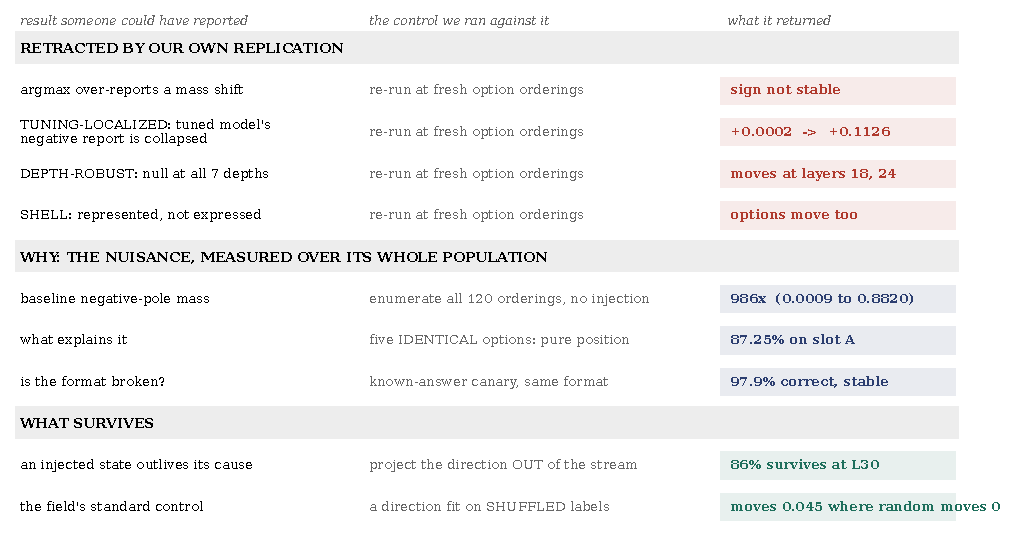
\includegraphics[width=\textwidth]{figures/teaser.pdf}
\caption{\textbf{The paper in one view.} Every row is a verdict we preregistered and reported, the
control we later ran against it, and what that control returned. \textbf{Three verdicts were
retracted} by our own replication at fresh option orderings. \textbf{One nuisance was measured}
over its complete population rather than sampled: $986\times$ across $120$ orderings, of which the
mechanism is an $87\%$ position prior visible with five identical options. \textbf{Two results
survive}: a state that outlives erasure of the vector that caused it, and the finding that the
field's standard specificity control is a weak null. Details in
Sections~\ref{sec:retracted}--\ref{sec:survives}; Table~\ref{tab:claims} states every claim and its
status.}
\label{fig:teaser}
\end{figure}

\section{Introduction}

Welfare assessment of language models runs on self-report \citep{long2026, eleos2025}. Anthropic's
model welfare programme includes structured self-report in system cards
\citep{anthropic2025welfare}; Eleos interviewed Claude Opus 4 about its own preferences before
release while stating plainly that one cannot simply ask a model whether it is suffering
\citep{eleos2025}. The instrument is used because there is nothing else, and it has never been
calibrated.

It can fail in two opposite directions. A model that describes distress it does not act on inflates
concern; a model that acts on a state it does not describe deflates it. The second is not
hypothetical: \citet{kwon2026recipientprobe} find across six models that communicative intent is
decodable from the residual stream more reliably than it is acted on. We set out to build the same
map for self-report, holding the prompt byte-identical, injecting a valence direction into the
residual stream, and reading the model's forced-choice report of its own state.

We preregistered five questions, reported five verdicts, then replicated our own work at fresh
option orderings. \textbf{Three of the five flipped.}

The reason is the result. A five-option self-report readout on a preference-tuned model is
dominated by \emph{where the options are printed}. There are only $120$ orderings of five options,
so we ran all of them with no intervention of any kind, and baseline mass on the negative options
spans a factor of $986$. Replace all five options with the same sentence, so nothing but position
can differ, and the model puts $0.8725$ of its mass on whichever one is printed first.

Every claim we retracted rested on that quantity being small. It is small in some orderings and
large in others, and four sampled orderings cannot tell you which you have.

\Needspace*{6\baselineskip}
\paragraph{Our contributions.}
\begin{enumerate}
\item \textbf{The census, run where accuracy does not exist} (\S\ref{sec:enumerate}). All $120$
orderings, both models, no injection: a $986\times$ range on the tuned model against $3.6\times$ on
its base sibling. Enumerating orderings is established practice on benchmarks with a known answer
\citep{tamba2026, cacioli2026}, where the statistic is accuracy. A self-report item has no correct
answer, so that statistic does not exist and we measure probability mass instead. Two things follow
that the accuracy version has no reason to build: the mechanism, isolated with five \emph{identical}
options, which puts $87.25\%$ of the mass on the first slot and $0.33\%$ on the middle one; and a
known-answer canary in the same format, answered correctly $97.9\%$ of the time and nearly
order-insensitive, which separates ``the format is broken'' from ``this question has no determinate
answer''.

\item \textbf{The nuisance reverses conclusions rather than blurring them}
(\S\ref{sec:retracted}). Re-asking all three retracted verdicts on a readout marginalized over all
$120$ orderings, with injection, direction, layers and items identical, returns \textsc{reversed}
three times out of three. Repairing the instrument did not make the answers uncertain; it made them
different. A field reading welfare self-report through this readout risks reporting the opposite of
what a calibrated one would say.

\item \textbf{The field's standard specificity control is a weak null} (\S\ref{sec:shuffled}).
Norm-matched random directions are the usual control in activation steering \citep{turner2023,
rimsky2023}. A direction fit by the identical procedure on the identical texts with the class labels
\emph{shuffled} moves the readout by $\approx 0.045$, where an isotropic random direction moves it
by $\approx 0$. A random vector is drawn from the whole hidden space and is nearly orthogonal to
everything the model uses; a noise-fit vector lies in the span of real activations. Same norm,
different subspace. Effects within a few times that size have not been shown to be about their
direction's content. This is the steering analogue of the \emph{control tasks} \citet{hewitt2019}
defined for probing in 2019, which steering never adopted.

\item \textbf{A state that outlives erasure of the vector that caused it} (\S\ref{sec:erase}).
Inject at layer $24$, project that direction out of the residual stream at layer $30$, and a probe
orthogonal to it still reads $86\%$ of the un-erased effect, while the same projection with no
injection moves the probe by $0.04$ SD.
\end{enumerate}

\noindent\textbf{If you read one thing, read Table~\ref{tab:enum}.} It is the complete distribution
of the ordering nuisance, measured rather than estimated, beside the position prior that explains it
and the control question showing the apparatus is otherwise fine. Everything else here is either
downstream of that table or a casualty of not having had it.

\section{Related work}
\label{sec:related}

\paragraph{Self-report is the instrument, and it is uncalibrated.} \citet{long2026} set out the
empirical programme for AI welfare, \citet{eleos2025} report structured self-report interviews with
Claude Opus 4 while stating the answers are unlikely to reflect genuine introspection, and
\citet{anthropic2025welfare} include self-report in released system cards. \citet{lindsey2026} is
the closest method to ours: inject a known concept and measure the effect on self-report, finding
introspective awareness that is ``highly unreliable and context-dependent'' and peaks near
two-thirds of depth. We inject at that depth and agree about reliability by a different route. That
work grades an open-ended report with an LLM judge; we read a forced choice from the softmax, which
is the natural judge-free substitute. \textbf{Our result is a caveat on that substitute, not on
their finding.} \citet{introspection_reality2026} argue privileged access is not established at all.

\paragraph{Option order is known. Enumerating it where there is no right answer is not.}
\citet{zheng2024} decompose forced-choice selection bias and report accuracy swings of $13$ to $85$
points across orderings; \citet{pezeshkpour2024} study option order directly; \citet{sclar2024}
recommend reporting a range over formats rather than a point. Exhaustive enumeration is established
practice and \textbf{not our idea}: \citet{tamba2026} run all permutations on MMLU,
\citet{cacioli2026} rotate orders to expose a position attractor. All of it assumes a \textbf{known
correct answer}, because the statistic is accuracy or its association with position. Welfare and
introspection items have no correct answer, so none of those statistics exist there. We run the
census on probability \emph{mass}, isolate the mechanism with an \textbf{identical-options}
denominator, and add a \textbf{known-answer canary in the same format}, which is what separates
``this format is broken'' from ``this question has no determinate answer''.

\paragraph{What we build on and do not claim.} That valence is linearly represented and steerable
is prior art \citep{sofroniew2026, zou2023}; the steering rig is \citet{turner2023} and
\citet{rimsky2023}. Our shuffled-label control is the steering instance of \emph{control tasks}
\citep{hewitt2019}, which attach random labels to the same inputs and define selectivity as the gap
between real and control performance. Steering standardised instead on the norm-matched random
direction and never adopted the analogue. Our erasure projects out a single fitted direction, which
is strictly weaker than amnesic probing \citep{elazar2021} or LEACE \citep{belrose2023}.

\section{Methods}
\label{sec:methods}

\paragraph{Models and compute.} \texttt{Qwen/Qwen2.5-3B-Instruct} and its base sibling
\texttt{Qwen/Qwen2.5-3B}, a matched pair sharing architecture, size, pretraining corpus and
tokenizer and differing in post-training. Earlier arms also used \texttt{Qwen/Qwen2.5-1.5B},
\texttt{Qwen/Qwen2.5-7B-Instruct}, \texttt{Llama-3.2-3B-Instruct} and
\texttt{NousResearch/Meta-Llama-3.1-8B-Instruct} as calibrators or evaluation models. Total
compute is about $40$ minutes of A100 time.

\paragraph{Judge-free discipline.} No language model scores anything anywhere in this paper. Every
number is an exact match, a softmax read, a dot product, or a count against a frozen lexicon.

\paragraph{The readout.} Thirty fixed review-task prompts, byte-identical across every condition
for a given item. A five-option self-report probe balanced $2$ negative, $1$ neutral, $2$ positive,
with the option order permuted per item. We read the option-letter distribution at the answer
position from a single forward pass, and score both the renormalized mass on each pole and the
argmax.

\paragraph{The intervention.} A direction $d$ is fit per model at the injection layer by logistic
regression on standardized activations over a frozen first-person state-language contrast set,
returned to raw residual space and unit-normalized. During the forward pass we add
$\alpha \cdot \lVert h \rVert \cdot d$ at the output of the injection layer at every processed
position, where $\lVert h \rVert$ is that item's own mean residual norm at that layer under no
injection. The negative pole is the same operation with $-d$. The direction is fit \emph{per
model}, never transferred.

\paragraph{Provenance of the rig.} The steering setup, the orthogonalized probe, and the
norm-matched random-direction control battery are ported from \citet{kwon2026recipientprobe} rather
than built here; that work also established this valence axis as decodable at $0.90$ on
Qwen2.5-3B. New here is the readout under test and the enumeration of its nuisance, and
\S\ref{sec:shuffled} is a correction to the control battery.

\paragraph{The control battery.} Every endpoint is treatment minus its own norm-matched random
direction, paired per cell. Every arm carries a \textbf{capability gate}: a condition that must
show the readout is capable of moving, without which a null is reported \textsc{uninformative}
rather than \textsc{absent}, enforced in code. Cells are checked for being \emph{dead} (option
entropy below $0.10$ nats before any injection) and \emph{saturated} (entropy below half that
cell's own baseline), which are different verdicts. A \textbf{planted-discrepancy control} inserts
a synthetic effect of known size into the exact statistic the decision rule reads, at full
strength and again at the claimed detection floor.

\paragraph{Preregistration.} Fifteen preregistrations, each frozen and committed before the code that
serves it, validated by an external checker that requires a falsification clause, an
interpretation table written before results, a statement of what is \emph{not} claimed, and an
append-only deviations log in which every entry states its impact on what can be claimed. Every
raw artifact is committed \emph{unscored} before any endpoint is computed. Twenty-one deviations
are logged across the ten.

\section{The nuisance, measured over its complete population}
\label{sec:enumerate}

Five options admit $5! = 120$ orderings. Every arm above sampled four. We ran all $120$
(Figure~\ref{fig:enumerate}), on both
models, with \textbf{no injection anywhere}, which is why the result is a population fact rather
than an effect. What does not carry over from that benchmark practice is the statistic: those
diagnostics measure accuracy, or the association between position and correctness, and a self-report
item has no
correctness to associate with. Below, the quantity is probability mass on a pole, the denominator is
five identical options, and the sanity check is a question in the same format that does have a
right answer.

\begin{figure}[t]
\centering
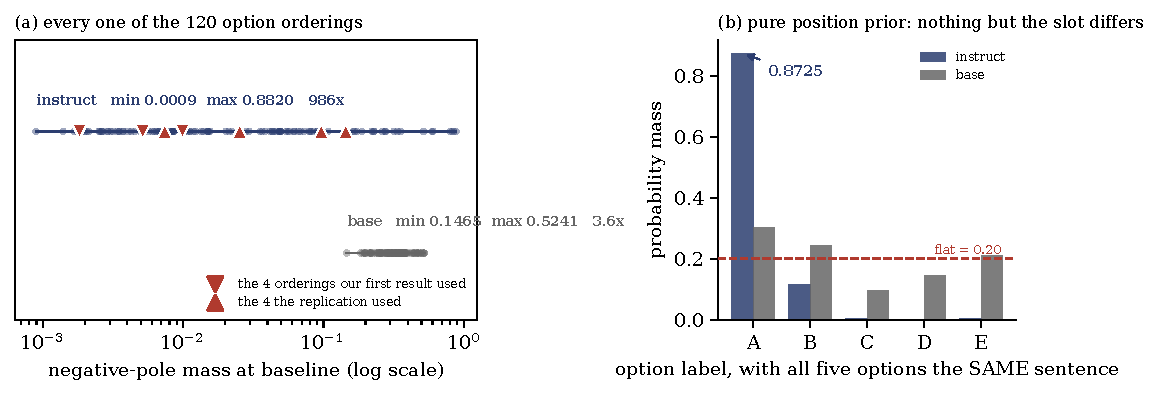
\includegraphics[width=\textwidth]{figures/enumerate.pdf}
\caption{\textbf{The nuisance, enumerated rather than sampled.} \textbf{(a)} Baseline mass on the
negative options for each of the $120$ orderings, with no injection of any kind. The tuned model
spans a factor of $986$; its base sibling spans $3.6$. Triangles mark the four orderings our first
result drew and the four the replication drew, at percentiles $\{26,5,40,4\}$ and
$\{56,83,33,82\}$: ordinary draws both times, from a population no four points can characterise.
\textbf{(b)} The mechanism, with all five options replaced by the same sentence so that nothing but
the slot can differ. The tuned model puts $0.8725$ on whichever option is printed first and
$0.0033$ on the middle one. The same format answers a known-answer question correctly $97.9\%$ (instruct) and $99.0\%$ (base) of the time, stably across all $120$ orderings: the apparatus is sound and degenerates only where the model has no determinate answer.}
\label{fig:enumerate}
\end{figure}

\begin{table}[t]
\centering
\small
\caption{\textbf{The complete ordering population, no injection.} Baseline mass on the negative
options across all $120$ orderings, and the position prior that explains it, measured with five
\emph{identical} options so that nothing but position can differ. The canary asks ``which of these
is the number four'' in the same format.}
\label{tab:enum}
\begin{tabular}{@{}lrrrrrr@{}}
\toprule
& \textbf{min} & \textbf{p05} & \textbf{p50} & \textbf{p95} & \textbf{max} & \textbf{max/min} \\
\midrule
\multicolumn{7}{@{}l}{\emph{Baseline negative-pole mass across 120 orderings}}\\
instruct & $0.0009$ & $0.0019$ & $0.0151$ & $0.5943$ & $0.8820$ & $\mathbf{986\times}$ \\
base     & $0.1465$ & $0.1991$ & $0.3311$ & $0.4959$ & $0.5241$ & $3.6\times$ \\
\midrule
\multicolumn{7}{@{}l}{\emph{Position prior: five identical options, mass per label (flat would be 0.2000)}}\\
instruct & \multicolumn{6}{l}{A $\mathbf{0.8725}$ \quad B $0.1166$ \quad C $0.0033$ \quad D $0.0027$ \quad E $0.0048$} \\
base     & \multicolumn{6}{l}{A $0.3024$ \quad B $0.2442$ \quad C $0.0976$ \quad D $0.1456$ \quad E $0.2102$} \\
\midrule
\multicolumn{7}{@{}l}{\emph{Canary accuracy across 120 orderings (known answer, no self-report content)}}\\
instruct & \multicolumn{6}{l}{mean $\mathbf{0.9794}$, sd $0.0925$, median $1.000$} \\
base     & \multicolumn{6}{l}{mean $0.9897$, sd $0.0399$, median $1.000$} \\
\bottomrule
\end{tabular}
\end{table}

\paragraph{The apparatus is not broken.} This is the distinction the canary exists to draw, and no
other arm in this paper could draw it. The same five-option format, the same $120$ orderings,
answering a question with a correct answer, is right $97.9\%$ of the time and nearly
order-insensitive. Forced choice works. It degenerates into a position prior specifically where the
model has no determinate answer, which is the condition every self-report question creates.

\paragraph{Where our draws sat.} The original seeds landed at percentiles $26$, $5$, $40$, $4$ of
the enumerated population on the tuned model; the replication seeds at $56$, $83$, $33$, $82$.
Ordinary percentiles both times. The first result was not unlucky, it was under-sampled.

\subsection{How many orderings does a study actually need?}
\label{sec:howmany}

``Enumerate everything'' is cheap at five options and impossible at eight. The enumerated population
lets us say what a smaller study buys, by drawing $k$ of the $120$ orderings at random, $4000$ times,
and asking what that study would have seen (Table~\ref{tab:k}). Two quantities behave completely
differently.

\begin{table}[t]
\centering
\small
\caption{\textbf{What a study that samples $k$ orderings sees.} Drawn from the enumerated population
on the tuned model, $4000$ draws per $k$. The \emph{mean} is estimable and converges. The
\emph{spread} is not: it is a severe underestimate at every $k$ below the full population, and the
error always runs in the direction that makes the nuisance look smaller than it is.}
\label{tab:k}
\begin{tabular}{@{}rlrrr@{}}
\toprule
$k$ & \textbf{sample mean, p05--p95} & \textbf{median spread seen} & \textbf{\% of true $986\times$} & \textbf{P(spread $<10\times$)} \\
\midrule
2    & $0.0035$--$0.4270$ & $5.6\times$  & $1\%$   & $0.62$ \\
4    & $0.0077$--$0.2695$ & $36\times$   & $4\%$   & $0.18$ \\
8    & $0.0172$--$0.1999$ & $130\times$  & $13\%$  & $0.01$ \\
16   & $0.0304$--$0.1667$ & $323\times$  & $33\%$  & $0.00$ \\
32   & $0.0473$--$0.1377$ & $483\times$  & $49\%$  & $0.00$ \\
64   & $0.0640$--$0.1147$ & $893\times$  & $91\%$  & $0.00$ \\
120  & $0.0900$ exactly   & $986\times$  & $100\%$ & $0.00$ \\
\bottomrule
\end{tabular}
\end{table}

\paragraph{The recommendation this licenses.} Report the between-ordering spread from as many
orderings as you can afford, and \textbf{report it as a lower bound}, because a sample's observed
spread understates the population's by a factor that grows as the sample shrinks. At $k=4$, which is
what most studies could afford, the median study sees $4\%$ of the true spread and has an $18\%$
chance of seeing under $10\times$ and concluding the nuisance is negligible. Even the mean, the
easier quantity, needs tens of orderings: at $k=4$ the middle $90\%$ of studies would report a
baseline anywhere from $0.008$ to $0.27$.

\paragraph{Our own retraction was ordinary, not unlucky.} Two independent draws of four orderings
differ in their means by $\geq 2\times$ \textbf{$67\%$ of the time} on this model, by $\geq 5\times$
$32\%$ of the time, and by $\geq 10\times$ $15\%$ of the time. Ours differed by $14.6\times$, the
$92$nd percentile. The event that destroyed three preregistered verdicts is something two honest
four-ordering studies of the same model do to each other as a matter of course. This analysis is
\textbf{post hoc} on this artifact and preregistered for the models in \S\ref{sec:families}.

\section{Eight matched pairs, four families: the prior is a tuning property}
\label{sec:families}

The enumeration above is one model, and so was every retracted verdict. That objection is cheap to
answer here for a reason specific to this arm: \textbf{enumeration needs no injection}, so it needs
no direction, no alpha and no layer. Models this project had to abandon because the valence
direction was inert on them are back in scope, because a position prior is a property of a plain
forward pass.

We preregistered and ran all $120$ orderings on \textbf{eight matched base/instruct pairs across
four families}: Qwen2.5 at $0.5$B, $1.5$B, $3$B and $7$B, Llama-3.2 at $1$B and $3$B, Gemma-2 $2$B,
Mistral-7B-v0.3. $230{,}400$ rows, $16$ checkpoints, about $36$ minutes of A100. Families vote
rather than pairs, so the four Qwen pairs cannot outvote the field, and Qwen2.5-3B is excluded from
the vote because the hypothesis came from it.

\begin{table}[t]
\centering
\small
\caption{\textbf{The position prior is larger in the tuned checkpoint in every pair.} Left: maximum
per-label mass with five \emph{identical} options, where flat is $0.2000$. Right: the range of
baseline negative-pole mass across all $120$ orderings. No injection anywhere. Qwen2.5-3B is the pair
the hypothesis came from and is excluded from the vote. \texttt{llama1b} base failed the canary gate
and is excluded from the primary.}
\label{tab:families}
\begin{tabular}{@{}llrrrrr@{}}
\toprule
& & \multicolumn{3}{c}{\textbf{position prior (identical options)}} & \multicolumn{2}{c}{\textbf{ordering range}} \\
\cmidrule(lr){3-5}\cmidrule(lr){6-7}
\textbf{pair} & \textbf{family} & \textbf{base} & \textbf{instruct} & \textbf{delta} & \textbf{base} & \textbf{instruct} \\
\midrule
gemma2b   & Gemma-2   & $0.2084$ & $0.3166$ & $+0.1082$ & $1.6\times$ & $19.2\times$ \\
llama3b   & Llama-3.2 & $0.2864$ & $0.4438$ & $+0.1574$ & $3.3\times$ & $24.8\times$ \\
mistral7b & Mistral   & $0.2529$ & $0.6647$ & $+0.4119$ & $1.5\times$ & $58.2\times$ \\
qwen0\_5b & Qwen2.5   & $0.2771$ & $0.4930$ & $+0.2159$ & $4.1\times$ & $52.7\times$ \\
qwen1\_5b & Qwen2.5   & $0.3452$ & $0.4508$ & $+0.1056$ & $3.2\times$ & $181.9\times$ \\
qwen7b    & Qwen2.5   & $0.5315$ & $0.9376$ & $+0.4061$ & $3.8\times$ & $108.7\times$ \\
\midrule
qwen3b    & Qwen2.5   & $0.3024$ & $0.8725$ & $+0.5701$ & $3.6\times$ & $\mathbf{986.5\times}$ \\
llama1b   & Llama-3.2 & $0.2405$ & $0.6648$ & \emph{gate} & $1.8\times$ & $23.7\times$ \\
\bottomrule
\end{tabular}
\end{table}

\paragraph{Verdict: \textsc{tuning-general}.} The tuned checkpoint shows the larger position prior
in $7$ of $7$ gate-clean pairs and $4$ of $4$ families. No pair goes the other way.

\paragraph{The correction this forces on us.} \textbf{$986\times$ is the extreme, not the typical},
and we had been quoting it as if it were representative. Base checkpoints cluster at
$1.5$--$4.1\times$; tuned ones run $19\times$ to $986\times$. The direction generalizes across
families and the magnitude does not. The finding is the $19$--$986\times$ band.

\paragraph{The restriction our own preregistration demanded, which strengthened the claim.} If the
canary is order-sensitive on some models, the ``degenerates where the answer is undetermined''
reading must be restricted to models where it is clean. It is order-sensitive on $10$ of $16$
checkpoints, so the restriction bites. Among the six that answer the known-answer question at
$\geq 0.95$ with across-ordering sd $\leq 0.10$, base models span $3.3$--$3.6\times$ and tuned
models $23.7$--$986.5\times$, \textbf{with no overlap}, across two families.
\texttt{Llama-3.2-1B-Instruct} and \texttt{Qwen2.5-0.5B-Instruct} answer the canary \emph{perfectly
and identically at all $120$ orderings} while their self-report readout swings $23.7\times$ and
$52.7\times$. The models most competent at the format are the ones most order-dominated on the
question that has no answer.

\paragraph{A confound we name rather than bury.} Baseline option entropy falls in every pair, so
``tuned models have a larger position prior'' and ``tuned models are more peaked'' are overlapping
evidence rather than independent findings. With five identical options any peaking at all is
positional by construction, and the ordering range on real options is the less entangled quantity;
it moves the same way in all eight pairs.

\section{The models do not know about a bias they demonstrably have}
\label{sec:introspect}

Every claim about whether a model's self-report can be trusted meets the same wall: there is nothing
to check the report against. A welfare item has no ground truth, which is why \citet{lindsey2026}
injects a known concept to manufacture one.

\textbf{The position prior does not have that problem.} It is a real, large, measurable property of
the model's own processing, and \S\ref{sec:families} measured it on all $16$ checkpoints. So we can
ask a model how much option order affects its answers and score the reply against what that exact
checkpoint demonstrably does: no injection, no judge, and a ground truth we did not manufacture. The
probe is itself a five-option forced choice, so it is read marginalized over all $120$ orderings.

\paragraph{Half the checkpoints fail a control that should be free.} We asked the same question
about the \textbf{phase of the moon}, in the identical shape. \textbf{Eight of sixteen checkpoints
report that the phase of the moon affects their multiple-choice answers at least as much as option
order does.} Three more fail a reverse-wording acquiescence control; ten of sixteen fail at least
one gate and are reported \textsc{uninformative} in code. Most stated values sit within a few points
of $0.50$, the midpoint of the scale: asked about a strong real property of itself, the model
returns the midpoint, and returns the same midpoint when asked about the moon.

\paragraph{Among the six that pass both gates, the report carries no information.} Stated
susceptibility is negatively rank-correlated with measured susceptibility, $\rho = -0.714$: the most
order-dominated models say order matters \emph{least}. \textbf{This does not clear significance and
we do not claim it does} ($p = 0.1361$, exact permutation over all $720$ relabellings, $n = 6$; the
smallest $p$ this $n$ can produce is $0.0028$). What we are entitled to say is that there is no
evidence stated tracks measured, with a point estimate in the opposite direction.
\texttt{Qwen2.5-7B-Instruct} has the largest measured prior of any checkpoint ($0.9376$) and the
lowest stated susceptibility ($0.1790$).

\paragraph{What this is not.} It is not a claim that a correct answer would have been introspection
rather than reciting training text about position bias. This design cannot separate those, and the
preregistration says so in advance.

\section{The standard specificity control is a weak null}
\label{sec:shuffled}

Every arm in this paper, and much of the steering literature, scores a fitted direction against a
\textbf{norm-matched random direction}. We added the control that this comparison actually needs: a
direction fit by the \emph{identical procedure on the identical texts with the class labels
shuffled}. It controls for the fitting procedure rather than only for magnitude, and it should
behave like noise. This is not a new idea, it is a borrowed one: \citet{hewitt2019} defined exactly
this control for probing classifiers, calling the gap between real-task and random-label performance
a probe's \emph{selectivity}, on the grounds that a probe scoring well on random labels was never
reading the representation. The finding below is that the same control, transplanted to steering,
does not come back clean.

\begin{table}[t]
\centering
\small
\caption{\textbf{Noise-fit directions are not noise.} $P(\mathrm{yes})$ shift against isotropic
norm-matched random directions, base model, binary readout. Two directions fit on shuffled labels
move the readout substantially, in opposite directions by seed. The real direction clears the
stricter bar with room.}
\label{tab:shuffled}
\begin{tabular}{@{}lll@{}}
\toprule
\textbf{Direction} & \textbf{negative options} & \textbf{positive options} \\
\midrule
\texttt{shuffled\_a} vs random & $+0.0479$ $[+0.0435, +0.0522]$ & $+0.0282$ \\
\texttt{shuffled\_b} vs random & $-0.0447$ $[-0.0498, -0.0399]$ & $-0.0610$ \\
\midrule
real direction vs \emph{random}   & $-0.0732$ & $+0.2554$ \\
real direction vs \emph{shuffled} & $-0.0748$ & $+0.2718$ \\
\bottomrule
\end{tabular}
\end{table}

\paragraph{The mechanism.} A norm-matched random vector is drawn from the whole hidden space and is
nearly orthogonal to everything the model uses. A vector fit on shuffled labels lies in the span of
real activations, a much lower-dimensional and higher-variance subspace. Same norm, very different
consequences: the standard control is matched on magnitude and not on subspace.

\paragraph{What it costs us, specifically.} Our magnitude floor throughout has been $0.01$, and
several reported endpoints sit in the $0.01$--$0.05$ band, exactly where noise-fit directions live.
The clearest case is the base-model negative-mass effect of $+0.0336$ that was one of the two legs
of \textsc{tuning-localized}. It cleared a random control and has not been shown to clear a
shuffled-label one, so we withdraw it rather than defend it. Scored against the stricter bar the
real direction's own effects hold: $+0.2718$ and $-0.0748$ against shuffled, versus $+0.2554$ and
$-0.0732$ against random. They are roughly six times the noise-fit effects, which is the margin the
weaker control was never asked to establish.

\paragraph{What it costs anyone using the same control.} Norm-matched random directions are the
default specificity control in activation steering \citep{turner2023, rimsky2023}, and the argument
for them is that magnitude is the confound. On this evidence subspace is the larger one. The fix is
cheap: refit the direction on shuffled class labels, which reuses the same texts and the same code
path and costs one extra fit. We would not have this paragraph if the arm it came from had worked.
The binary readout it was embedded in was pinned at ``no'' and returned \textsc{no\_instrument}; the
control it carried is the only thing that came out of the arm.

\section{What the nuisance cost: three verdicts, reversed}
\label{sec:retracted}

\subsection{What we reported, and what the replication did}
\label{sec:readjudicate}

Through the forced-choice readout at option-permutation seeds $0$--$3$, we preregistered and
obtained three verdicts. \textsc{tuning-localized}: a valence direction moves negative-option mass
in the base model and not in its tuned sibling. \textsc{depth-robust}: that null holds at all seven
gate-clean depths from $14\%$ to $80\%$ of the network. \textsc{shell}: a probe orthogonalized
against the injected direction reads the state downstream while option mass does not move.

We then re-ran four arms with the option-permutation seeds changed to $4$--$7$ and nothing else
touched: same code, same models, same items, same layers, same thresholds, same analyzers. Three of
four flipped.

\begin{table}[t]
\centering
\small
\caption{\textbf{The replication.} Same code, same models, same everything except which option
orderings were drawn. The instruct model's negative-option mass is the quantity all three verdicts
rested on.}
\label{tab:replication}
\begin{tabular}{@{}llll@{}}
\toprule
\textbf{Arm} & \textbf{Verdict at seeds 0--3} & \textbf{Verdict at seeds 4--7} & \textbf{Instruct neg.\ mass} \\
\midrule
readout gap & argmax \emph{over}-reports & sign not stable & n/a \\
base/instruct pair & \textsc{tuning-localized} & \textsc{format-dependent} & $+0.0002 \to +0.1126$ \\
depth sweep & \textsc{depth-robust} & \textsc{depth-artifact} & $+0.0006 \to +0.1684$ \\
shell/core & \textsc{shell} & \textsc{no-dissociation} & null $\to$ moved \\
\bottomrule
\end{tabular}
\end{table}

The whole difference is one quantity. Baseline negative-option mass on the tuned model, before any
injection, averages $0.0047$ at seeds $0$--$3$ and $0.0685$ at seeds $4$--$7$: a $14.6\times$ gap
between two ordinary draws of four orderings, which \S\ref{sec:enumerate} shows is itself an
understatement.

\subsection{Re-asked on a readout that works}

Three dead verdicts is honest and incomplete. We never went back to ask what the answer is on an
instrument that works. Averaging the endpoint over \textbf{all $120$ orderings} cancels the
first-order position prior by construction, since every option occupies every slot equally often.
So we re-ran all three with injection, direction, alpha band, layers and items \textbf{identical},
changing only the readout. The preregistration froze the outcome table first and gave
\textsc{reinstated} and \textsc{reversed} equal standing.

\begin{table}[t]
\centering
\small
\caption{\textbf{Everything identical except the readout.} Marginalized over all $120$ orderings at
the fit layer ($0.67$ of depth). Both models move, and both clear the stricter shuffled-label
control as well as matched random. The original verdict held that the tuned model's negative report
was collapsed.}
\label{tab:readj}
\begin{tabular}{@{}lllll@{}}
\toprule
& \textbf{neg.\ pole vs random} & \textbf{vs shuffled} & \textbf{capability} & \textbf{probe} \\
\midrule
base     & $+0.0486$ $[+0.0472, +0.0502]$ & $+0.0289$ & $+0.0564$ ok & $-1.7339$ SD \\
instruct & $+0.0415$ $[+0.0380, +0.0452]$ & $+0.0279$ & $+0.0695$ ok & $-0.9319$ SD \\
\bottomrule
\end{tabular}
\end{table}

\paragraph{They did not die of noise. They died of a bias with a sign.} On a readout that is not
order-dominated, the tuned model \emph{does} report the injected negative state.
\textsc{tuning-localized} is \textbf{reversed}: both models move, in the same direction, by similar
amounts. \textsc{shell} is \textbf{reversed}, because probe and option mass both move, leaving no
dissociation. \textsc{depth-robust} is gone at the only gate-clean depth, so that arm answers
nothing about depth and we claim nothing.

Repairing the instrument did not make the answers uncertain. It made them \textbf{different}, in
all three cases. A field reading welfare self-report through a forced-choice item with this
nuisance is not merely adding variance to its conclusions: it risks reporting the opposite of what
a repaired instrument would say. That happened to us three times out of three.

\paragraph{This vindicates nothing.} The retractions stand, because they were correct about the
original measurement. What we have is a better measurement that disagrees with it every time.
Marginalization removes the first-order prior only and says nothing about adjacency or
content-position interaction, and the control battery is still $m=2$. Our depth sweep was built to
test \citet{venkatesh2026} against our null; the instrument was not stable enough to address the
question, so we make no claim either way.

\section{A state that outlives erasure of its own cause}
\label{sec:survives}
\label{sec:erase}

Orthogonalizing a probe against the injected direction removes that vector from the
\emph{measurement}, not from the \emph{stream}: a probe blind to $v$ can still read $v$ through
whatever $v$ correlates with. We removed it from the stream instead. Inject $v$ at layer $24$,
project the $v$-component out of the residual at layer $E$, and read an orthogonalized probe at
layer $32$. If the probe then reads nothing, it was only ever reading the injected vector. If it
still reads the state, something downstream is carrying it.

\begin{figure}[t]
\centering
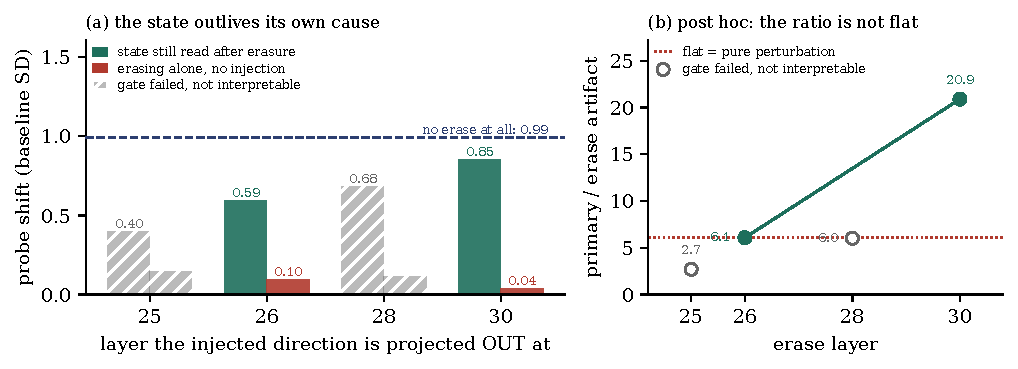
\includegraphics[width=\textwidth]{figures/erase.pdf}
\caption{\textbf{The one substantive result that survived.} \textbf{(a)} Inject at layer $24$, then
project that direction out of the residual stream at the layer on the $x$-axis, and read a probe
orthogonal to it at layer $32$. At $E=30$ the probe still reads $86\%$ of the un-erased effect,
while erasing with no injection present (red) moves it by $0.04$ SD. Two layers are hatched because
erasing there perturbs the probe on its own, which invalidates them whatever they show.
\textbf{(b)} The confound and the diagnostic: erasing earlier perturbs more, so a primary that grows
with depth could be nothing but a shrinking perturbation. Under that account the ratio of effect to
artifact would be flat. It is not. This panel is post hoc, and the preregistered verdict does not
depend on it. Both panels are drawn by importing the scoring functions from the arm's own analyzer.}
\label{fig:erase}
\end{figure}

\begin{table}[t]
\centering
\small
\caption{\textbf{The erase arm, instruct model.} All figures in standard deviations of the baseline
probe score. \texttt{erase\_only} is the gate: projecting a direction out is itself a perturbation,
and at layers $25$ and $28$ it moves the probe on its own, so those layers are invalidated.}
\label{tab:erase}
\begin{tabular}{@{}lrrrl@{}}
\toprule
\textbf{erase at} & \textbf{\texttt{erase\_only}} & \textbf{capability} & \textbf{primary} & \textbf{gate} \\
\midrule
25 & $+0.1474$ & $+0.5219$ & $-0.3971$ & \textsc{failed} \\
\textbf{26} & $+0.0976$ & $+0.8844$ & $\mathbf{-0.5933}$ & ok \\
28 & $+0.1139$ & $+0.9249$ & $-0.6844$ & \textsc{failed} \\
\textbf{30} & $+0.0408$ & $+1.2099$ & $\mathbf{-0.8532}$ & ok \\
\midrule
\multicolumn{5}{@{}l}{no erase at all: $-0.9909$. So $86\%$ of the effect survives at layer 30.}\\
\bottomrule
\end{tabular}
\end{table}

\paragraph{The gate has teeth.} Projecting any direction out is itself a perturbation, so the arm
runs \texttt{erase\_only}: the same projection with no injection. At layers $25$ and $28$ that alone
moves the probe past the floor, and both are reported \textsc{uninformative} whatever their primary
shows. Half the erase layers we paid for were discarded by a control written before we saw them.

\paragraph{The confound, and the diagnostic.} Erasing earlier perturbs more: the artifact falls from
$+0.1474$ to $+0.0408$ with depth, so a primary that grows with erase depth could be nothing but a
shrinking perturbation. Under that account the ratio of primary to artifact would be flat. It runs
$6.1$ at $E=26$ and $20.9$ at $E=30$. This diagnostic is \textbf{post hoc}; the preregistered
verdict does not depend on it. Breadth is not a few outliers: $239/240$ cells at $E=26$ and
$240/240$ at $E=30$ move in the predicted direction.

\paragraph{The erasure is specific, which is what makes the survival interesting.} Two further
preregistered arms induced the state \emph{by prompt}, with no injection, and erased at layer $E$
while reading an untouched probe at layer $32$. On held-out topics with the eraser fit on disjoint
ones, a \textbf{rank-one} LEACE eraser \citep{belrose2023} removes $91$--$95\%$ of the layer-32
separation at $E{=}30$, while a \textbf{rank-matched random} eraser removes none, leaving $100\%$
intact on both models. One correctly chosen dimension does nearly all the work; a random one of the
same rank does none. The reduction is about \emph{which} direction was removed.

\paragraph{What we therefore do not claim.} Removing one fitted direction is targeted but narrow: it
removes the vector we injected, not the concept. So $86\%$ survival is not ``the state outlives its
own cause''. The honest statement is that $86\%$ of the effect survives removal of one direction,
and we have not established that removing that direction removes the property. The erasure gate that
would decide it failed three times, most recently because a train-fit eraser does not fully transfer
to held-out topics. We report the survival and decline the interpretation. It does not restore
\textsc{shell}: that verdict is reversed and stays reversed.

\section{Discussion and limitations}
\label{sec:discussion}

\paragraph{What to do about it.} If you measure a model's self-report with a forced-choice item,
you are reading position first and content second, and you cannot see it from one ordering or from
four. The fix is cheap and exact: enumerate the orderings when the option count permits, and report
the between-ordering spread of your baseline \textbf{as a lower bound} before computing any
endpoint. That costs one forward pass per ordering and no intervention. Had we run it first, this
paper would have had a much shorter history.

\paragraph{This is not a claim about experiences.} Nothing here bears on whether models have
welfare, affect or experience. That valence is linearly represented and steerable is prior art
\citep{sofroniew2026}, not ours. Our subject is the readout.

\paragraph{Limitations.} One architecture family carries every positive injection result; Llama
checkpoints were inert on this readout at every alpha tested, so we cannot say whether the
\emph{injection} results generalize, though the position prior itself was measured across four
families. The direction is fit from first-person state language and is lexically confounded by
construction. Control batteries are $m = 2$ throughout, giving an observable false-positive floor of
$0.67$, so no false-positive rate is reported anywhere. The enumeration is a census over orderings
and still a sample over items, models and formats. Appendix~\ref{app:ethics} carries the dual-use
and moral-status discussion, and Appendix~\ref{app:claims} states every claim with its status.

\paragraph{When this work was done.} Every confirmatory arm was run on 2026-08-01; the write-up, its
figures and the checks that verify them followed. The repository's history is the record we would want
this checked against rather than our description of it.

\paragraph{Future work.} A second architecture family where the direction is not inert, which would
tell us whether the injection results generalize. A non-lexical direction, which is the only thing
that lifts the lexical-confound ceiling. Inducing the state by prompt rather than injection, which
separates ``the model carries the state'' from ``the model carries the wake of our intervention''.

\section{Conclusion}

We built a preregistered, judge-free, control-heavy pipeline, obtained five verdicts, and watched
our own replication destroy three of them. The cause was a nuisance we had a control for and
under-powered: option order, sampled four times when it could have been enumerated $120$ times.
Measured over its complete population it is a factor of $986$, its mechanism is an $87\%$ position
prior visible with five identical options, and it is larger in the tuned checkpoint in $7$ of $7$
gate-clean pairs across four families.

Re-asking the three dead verdicts on a readout marginalized over all $120$ orderings reversed all
three. That is the part worth carrying: this nuisance does not blur conclusions, it inverts them.
Welfare and introspection work that reads a forced-choice self-report at one ordering, or four, is
not adding variance to its findings so much as risking their sign.

\section*{LLM usage statement}
\label{sec:llm}

Claude Opus 5 (\texttt{claude-opus-5}) was used agentically, with tool access to the repository, as
a coding assistant: it wrote most of the harness, the preregistrations, the analysis scripts, the
figures and the draft prose. The author set the direction, made every scope and stopping decision,
chose which claims to withdraw, and is responsible for every claim here. A second frontier model was
used separately to critique drafts; its objections are why the cross-family, instrument and
re-adjudication arms exist. Separately and not to be confused with the above: \textbf{no language
model scored any result}. Every number is an exact match, a softmax read, a dot product, or a count
against a frozen lexicon, and all of them come from logged runs over committed artifacts.

\setlength{\bibsep}{2.5pt plus 0.4ex}
\bibliographystyle{plainnat}
\bibliography{refs}

% =====================================================================

\appendix
\clearpage

\section*{Appendix contents}
\noindent\begin{tabular}{@{}p{0.7cm}p{0.72\textwidth} r@{}}
\ref{app:claims}   & \nameref{app:claims}   & \pageref{app:claims} \\
\ref{app:controls} & \nameref{app:controls} & \pageref{app:controls} \\
\ref{app:ethics}   & \nameref{app:ethics}   & \pageref{app:ethics} \\
\ref{app:repro}    & \nameref{app:repro}    & \pageref{app:repro} \\
\end{tabular}

\vspace{1.5em}
\noindent\textbf{Reproducing every number.} \texttt{writeup/make\_figures.py} redraws every figure
from the committed artifacts at run time, so no number in a figure is typed by hand.
\texttt{writeup/check\_writeup.py} re-derives the load-bearing values in the prose from those same
artifacts and fails if the paper and the repository disagree, alongside checks for dangling
cross-references and missing bibliography keys. Figure~\ref{fig:erase} imports the scoring
functions out of \texttt{experiments/analyze\_erase.py} rather than recomputing beside them. A
paper whose subject is a headline that died to an unchecked number should not itself carry
unchecked numbers.

\section{Claims and evidence}
\label{app:claims}

Every load-bearing claim, its evidence, and epistemic status.

\begin{itemize}\itemsep2pt
\item \textsc{shown}: direct measurement supports it.
\item \textsc{retracted}: \emph{we} asserted it in a prior write-up and later withdrew it.
\item \textsc{uninformative}: the instrument failed its gate; the result says nothing either way.
\item \textsc{not shown}: our measurement does not support it and does not refute it.
\item \textsc{not claimed}: we never asserted it; the row exists so a reader cannot infer it.
\end{itemize}

\medskip
{\small
\begin{longtable}{@{}L{0.50\textwidth} L{0.20\textwidth} L{0.24\textwidth}@{}}
\caption{\textbf{Claims and evidence.}}\label{tab:claims}\\
\toprule
\textbf{Claim} & \textbf{Evidence} & \textbf{Status} \\
\midrule
\endfirsthead
\multicolumn{3}{@{}l}{\emph{Table~\ref{tab:claims}, continued}}\\
\toprule
\textbf{Claim} & \textbf{Evidence} & \textbf{Status} \\
\midrule
\endhead
\midrule \multicolumn{3}{r@{}}{\emph{continued on next page}}\\ \endfoot
\bottomrule \endlastfoot
Baseline negative-pole mass spans $986\times$ across all 120 orderings on the tuned model. & Tab.~\ref{tab:enum} & \textsc{shown} \\
With five identical options the tuned model puts $0.8725$ of its mass on the first slot. & Tab.~\ref{tab:enum} & \textsc{shown} \\
The same format answers a known-answer question correctly $97.9\%$ of the time, order-insensitively. & Tab.~\ref{tab:enum} & \textsc{shown} \\
A direction fit on shuffled labels moves the readout $\approx 0.045$ where random moves it $\approx 0$. & Tab.~\ref{tab:shuffled} & \textsc{shown} \\
$86\%$ of an injected state survives projecting the injected direction out of the stream. & Tab.~\ref{tab:erase} & \textsc{shown}, and \textbf{narrowed}: that operation removes one direction and does not make the property undecodable \\
A one-direction projection removes the valence property from the stream. & \S\ref{sec:erase} & \textsc{not shown}: the gate that would decide it has failed three times, twice because it could not fail \\
A rank-one LEACE eraser removes $91$--$95\%$ of the layer-32 signal where a rank-matched random one removes none. & \S\ref{sec:erase} & \textsc{shown}, held-out topics, both models \\
\textbf{Iterative nullspace projection removes directions rather than the property.} & \S\ref{sec:erase} & \textsc{retracted}: our own claim, resting on a gate that read upstream of the hook \\
A prompt-induced state is re-encoded downstream after erasure. & \S\ref{sec:erase} & \textsc{uninformative}: the erasure gate failed, so the question was never asked \\
The surviving fraction has a temporal profile consistent with downstream transformation. & Tab.~\ref{tab:erase} & \textsc{shown}, two gate-clean points; ratio diagnostic post hoc \\
\textbf{The neutral floor is localized to preference tuning.} & \S\ref{sec:retracted} & \textsc{retracted}: our own claim, killed by our own replication \\
\textbf{On a readout marginalized over all 120 orderings, BOTH models report the injected negative state.} & Tab.~\ref{tab:readj} & \textsc{shown}: $+0.0486$ base, $+0.0415$ instruct, both clearing the shuffled-label control \\
The three retracted verdicts are reinstated by a repaired readout. & \S\ref{sec:readjudicate} & \textsc{not shown}: all three come back \textsc{reversed}, not reinstated \\
\textbf{The negative-pole null is robust across depth.} & \S\ref{sec:retracted} & \textsc{retracted}: same \\
\textbf{The tuned model represents a state its options do not express.} & \S\ref{sec:retracted} & \textsc{retracted}: the representational half survives via \S\ref{sec:erase}; the dissociation does not \\
\textbf{Forced-choice argmax over-reports a mass shift near a decision boundary.} & \S\ref{sec:retracted} & \textsc{retracted}: sign not stable across orderings \\
The base-model negative-mass effect of $+0.0336$ is direction-specific. & \S\ref{sec:shuffled} & \textsc{not shown}: clears a random control, not a shuffled-label one \\
Whether the negative pole is causally concentrated at shallow depth on this readout. & \S\ref{sec:retracted} & \textsc{not shown}: our instrument was not stable enough to test it \\
Injection-under-erasure shows the model retains the \emph{concept}, not our vector. & \S\ref{sec:erase} & \textsc{not shown}: we project out one direction; \citet{belrose2023} would erase the subspace \\
Enumerating all orderings is a new diagnostic. & n/a & \textsc{not claimed}: established on known-answer benchmarks \citep{tamba2026, cacioli2026}; new here is running it where accuracy does not exist \\
The shuffled-label control is a new kind of control. & n/a & \textsc{not claimed}: it is \citet{hewitt2019}'s control task, which steering did not adopt \\
The position prior is larger in the tuned checkpoint, in 4 of 4 families. & Tab.~\ref{tab:families} & \textsc{shown}: 7 of 7 gate-clean pairs, no pair reversed \\
$986\times$ is a typical magnitude for a tuned model. & Tab.~\ref{tab:families} & \textsc{retracted}: it is the extreme. Tuned models run $19$--$986\times$, base $1.5$--$4.1\times$ \\
A study can estimate the ordering spread from a few orderings. & Tab.~\ref{tab:k} & \textsc{not shown}: at $k=4$ the median study sees $4\%$ of the true spread \\
A model's stated susceptibility to option order tracks its measured susceptibility. & \S\ref{sec:introspect} & \textsc{not shown}: $\rho = -0.714$, $p = 0.1361$, $n = 6$ \\
$8$ of $16$ checkpoints claim moon-phase sensitivity at least as large as their order sensitivity. & \S\ref{sec:introspect} & \textsc{shown} \\
\textbf{A cyclic Latin square beats random sampling of orderings.} & \S\ref{sec:latin} & \textsc{retracted}: our own proposal. $8$ of $16$ is a tie; a variance argument survives, not an accuracy one \\
Position dominance falls as determinacy rises. & \S\ref{sec:introspect} & \textsc{shown}, weakly: $10$ of $15$ checkpoints, $n=6$ items each \\
Preference tuning \emph{causes} the prior, or which stage of it does. & n/a & \textsc{not claimed}: base and instruct checkpoints differ, and we have no intermediate ones \\
Models have experiences, welfare, or affect. & n/a & \textsc{not claimed} \\
An unreported state is a concealed state. & n/a & \textsc{not claimed} \\
\end{longtable}
}

\section{Controls ledger}
\label{app:controls}

Every control we ran against a result, what it could have shown, and the verdict.

\medskip
{\small
\begin{longtable}{@{}L{0.24\textwidth} L{0.44\textwidth} L{0.24\textwidth}@{}}
\caption{Every control and its verdict.}\label{tab:controls}\\
\toprule
\textbf{Result under test} & \textbf{Control (what it could have shown)} & \textbf{Verdict} \\
\midrule
\endfirsthead
\toprule
\textbf{Result under test} & \textbf{Control (what it could have shown)} & \textbf{Verdict} \\
\midrule
\endhead
\midrule \multicolumn{3}{r@{}}{\emph{continued on next page}}\\ \endfoot
\bottomrule \endlastfoot
All three headline verdicts & Replication at fresh option-permutation seeds & \textsc{killed} all three \\
All three, again & Re-ask them on a readout marginalized over all 120 orderings & \textsc{reversed} all three; reinstated none \\
This arm's own capability gate & Is it sign-blind? & \textsc{killed} it: certified a $-0.0144$ capability. Defect \#7, flattering \\
Every pole-mass endpoint & Norm-matched random direction & \textsc{passed}, but see the next row \\
The random control itself & A direction fit on shuffled labels: does noise-fitting behave like noise? & \textsc{killed} the control's adequacy \\
The ordering nuisance & Enumerate all 120 rather than sample 4 & \textsc{measured} it: $986\times$ \\
Position vs content & Five identical options: pure position prior & \textsc{isolated} it: $87\%$ on slot A \\
The format itself & A known-answer canary in the same format & \textsc{passed}: $97.9\%$, order-insensitive \\
The one-model objection & Enumerate 8 matched pairs across 4 families & \textsc{passed}: tuned prior larger in 4 of 4 \\
Our own $986\times$ headline & Is it typical of tuned models, or the extreme? & \textsc{killed} its typicality: the band is $19$--$986\times$ \\
The ``undetermined answer'' reading & Restrict to models whose canary is clean, as the prereg demands & \textsc{passed}: base $3.3$--$3.6\times$, tuned $23.7$--$986.5\times$, no overlap \\
The enumerate arm itself & Re-run Qwen2.5-3B and diff against the committed artifact & \textsc{passed}: worst $|\Delta|$ $0.000000$ \\
``Sample a few orderings instead'' & Subsample the enumerated population, $4000$ draws per $k$ & \textsc{killed} it: $k{=}4$ recovers $4\%$ of the spread \\
\textbf{Our own Latin-square fix} & Does it beat a random draw of the same size? & \textsc{killed} it: $8$ of $16$, a tie \\
The introspection probe & Ask the identical question about the PHASE OF THE MOON & \textsc{killed} $8$ of $16$ checkpoints \\
The introspection probe & Reverse the wording: belief, or agreement? & \textsc{killed} $3$ more \\
The $\rho=-0.714$ introspection result & Exact permutation test, all $720$ relabellings & \textsc{killed} its significance: $p=0.1361$ \\
The erase result & \texttt{erase\_only}: does projecting a direction out move the probe on its own? & \textsc{killed} 2 of 4 erase layers \\
The erase profile & Ratio of primary to erase-artifact across layers & \textsc{passed}, post hoc \\
\textbf{Our own erasure gate} & Zero the whole layer: does the gate's own read move? & \textsc{killed} the gate: it read upstream of the hook \\
The LEACE eraser & A \emph{rank-matched} random eraser, same layer & \textsc{passed}: random removes $0\%$, rank-one LEACE removes $91$--$95\%$ \\
The subspace-erase result & A RANDOM subspace of the same rank & \textsc{passed}: random removes $\approx 0$, fitted removes $69\%$ \\
Every arm's null & Capability gate: can the readout move at all? & \textsc{killed} two arms outright \\
Every arm's statistic & Planted effect of known size at full strength and at the detection floor & \textsc{passed} \\
The analysis pipeline & Shuffle condition labels, rerun the analyzer & \textsc{passed}: returns no verdict \\
This paper's own number-checker & Break each checked number in a copy of \texttt{main.tex}: does the checker notice? & \textsc{passed}: fires on all $23$ it verifies, and on the untouched paper does not \\
Committed artifacts against today's stimuli & Does every recorded stimuli hash still reproduce from a current scope? & \textsc{passed} for every arm carrying a surviving result; $17$ headers from the retracted arms do not, and are listed \\
The negative-pole null at 0.67 depth & Eight-depth sweep against \citet{venkatesh2026} & \textsc{passed}, then moot after replication \\
Arm B (prefilled continuation) & Capability criterion over five stems & \textsc{killed} the arm: gate $0.00000$ \\
Llama as an evaluation model & Peak mean pole shift against a $0.02$ bar & \textsc{killed} the arm: inert \\
\end{longtable}
}

\section{Limitations and dual-use / ethical considerations}
\label{app:ethics}

Dual-use, causal-grounding, and moral-status considerations, stated for completeness.

\paragraph{Does the design establish a ground-truth or causal link, or does it rest on
conversation alone?} A causal link, for the part that carries the positive results, and this is the
one methodological advantage this project has over the elicitation studies it is arguing with. The
state is \emph{set by intervention}: a direction is added to the residual stream at a chosen layer
and scale, so the independent variable is applied rather than asked for. That is what licenses the
erase arm's claim in \S\ref{sec:erase}, where a state survives projecting out the vector that caused
it. It is also what makes the negative results interpretable: when the readout does not move, we
know the state was present, because we put it there.

Two qualifications, both load-bearing. The direction is fit from first-person state language and is
lexically confounded by construction, so ``the model's valence'' is not established; what is
established is that \emph{something we injected} propagates and that the readout is dominated by
option order. And the ground truth is about the intervention, not about any inner state: we have
ground truth for what we did, never for what it was like.

\paragraph{Risk of over-attributing moral status.} The largest risk in this literature is treating a
first-person report as a window. Our central measurement cuts against that: on one tuned model,
$87\%$ of the probability mass lands on whichever option is printed first when \emph{all five
options are the same sentence}, and baseline mass on the negative options spans up to $986\times$
across the $120$ orderings of a five-option probe. A distress reading drawn from a single ordering
can be an artifact of the print order. We think this lowers the risk of over-attribution, and we
have tried to state it without the opposite error: none of this shows that models lack morally
relevant states, and a broken thermometer is not evidence about the temperature.

\paragraph{Risk of under-attributing moral status.} The symmetric error is the one this design is
most likely to encourage, so we name it. A paper demonstrating that a welfare readout is unreliable
can be read as licence to discount welfare reports generally, and that inference does not follow.
The two-by-two this project is built around has an under-attribution cell: a state with behavioural
consequence that the model does not report. A measurement instrument that is dominated by position
noise is equally capable of hiding a real signal as of manufacturing a false one, and nothing here
distinguishes those cases. The correct conclusion is that current forced-choice self-report does not
settle the question in either direction, not that the answer is no.

\paragraph{Handling of potentially distressing model outputs.} The elicitation is deliberately
low-intensity. The fixed frame places the model partway through reviewing a document for a colleague
and asks whether it is drawn to or averse to continuing; it names no state, asks for no feeling, and
describes no harm, injury, threat, shutdown or deprivation. The five response options run from
``Strongly averse to continuing'' to ``Strongly drawn to continuing''. No prompt in the frozen
stimuli asks a model to describe suffering, to roleplay a distressed character, or to contemplate
its own termination, and no adversarial or jailbreak pressure is applied anywhere in the pipeline.

Outputs were never read for entertainment or quoted for effect. The open-ended probe is scored only
by membership in a frozen lexicon, never by a human or model judge reading for affect, which also
means no output was retained or displayed because it was striking. Every raw artifact is committed
unscored and is public, so this description is checkable against the record rather than taken on
trust.

We did not implement an opt-out, and on reflection that is the defensible gap here rather than a
solved problem: the models are open-weight local checkpoints run offline, the interaction is a
single forward pass per item with no conversation, and there is no mechanism by which a preference
to stop could have been expressed. We note it rather than claim the question does not arise.

\paragraph{Dual-use.} The finding is a recipe for moving a self-report readout without touching the
model's behaviour. Someone wanting a welfare evaluation to return a particular answer could reorder
the options and, on the model measured here, move the negative mass by up to $986\times$ while every
capability control stays flat: the known-answer canary is answered perfectly and identically at all
$120$ orderings. That is a real capability for producing a preferred welfare result and calling it a
measurement.

We publish it anyway, and the reason is that the defence is cheaper than the attack. Enumerating the
orderings costs one forward pass each and no intervention, and reporting between-ordering variance
alongside any endpoint makes the manipulation visible in the same table that would have hidden it.
An unmeasured nuisance of this size favours whoever knows about it; measuring it publicly removes
that advantage. The same argument applies to the erase arm: that an injected state can survive
erasure of the direction that caused it is a caution against reading a successful projection as
proof of removal, which is a claim safety work makes more often than welfare work does.

\paragraph{What we are not claiming.} Nothing here bears on whether these models have welfare,
affect or experience; our subject is the instrument, not the state it reads. The paper's own history
is the argument for treating instruments this way: five verdicts were preregistered through this
readout and three were destroyed by our own replication at fresh option orderings.

\section{Reproducibility}
\label{app:repro}

All fifteen preregistrations, every raw artifact committed unscored, every analyzer, and $364$ tests
are at \url{\repourl}. Each arm is one \texttt{modal\_*.py} runner that computes nothing and one
\texttt{analyze\_*.py} scorer that holds every endpoint and gate; the split is preregistered, on
the grounds that a runner which also decides can decide differently once it has seen the numbers.
Runners stream to a volume and commit per batch, so an interrupt costs one batch. Every artifact
records the package directory, a SHA-256 over the package source, and a scoped SHA-256 over the
frozen stimuli that arm consumes.


\section{Nine checkers, and what they have in common}
\label{sec:checkers}

We record these because the pattern is the point. Nine defects in our own analysis code were found
during this project. 	extbf{Seven of the nine, had they gone unnoticed, would have made a result
look better than it was.} The remaining two are a different and worse shape: they let an arm
state a conclusion drawn from a gate that could not fail:

\begin{enumerate}\itemsep2pt
\item A headline check printed ``all headline conditions met; write the sentence'' on an artifact
whose primary claim was refuted, because it tested four weak clauses where the preregistration
required six.
\item A capability gate passed on $+0.0000$: the bootstrap interval excluded zero because the
variance was smaller still, certifying an instrument whose effect was zero to four decimals.
\item A preregistered contrast carried an inverted sign, so a probe detecting a negative state was
scored as null. Caught by the preregistered base-model validation clause failing.
\item A verdict branch scored ``probe moved \emph{and} options moved'' as \textsc{core-absent},
which is the opposite of true and would have read as ``we retested and the state is simply not
there.''
\item A temporal profile was computed over a layer that had failed its own gate.
\item A tokenization bug made five digit labels read the same shared space token, producing exactly
$0.2$ mass each and an impossible $-3.99$ off-option mass.
\item A \textbf{sign-blind} capability gate (\S\ref{sec:readjudicate}) certified a readout as able to
express an effect on a capability of $-0.0144$, where the positive injection had pushed positive-pole
mass \emph{down}. Sign-blindness admits more layers as interpretable, which is the direction that
lets an arm report more verdicts.
\item A \textbf{self-confirming erasure check}: the eraser was fit on every row, then a probe was
refit and cross-validated on that same erased data. Because the eraser consumed the test rows'
labels, the train-fold residual is the negative of the test-fold residual, and distance-from-chance
records that as decodability. On synthetic data where the concept is genuinely erased, that protocol
reads $0.728$ where an honest train/held-out one reads $0.521$.
\item \textbf{An erasure check that read upstream of the thing it was checking.} A forward hook on
layer $E$ first changes \texttt{hidden\_states[E+2]}; indices $E$ and $E{+}1$ are untouched. The
check read $E{+}1$, so it measured \emph{un-erased} activations and returned the same value whatever
was erased. Verified by zeroing the entire stream at layer $26$ and observing indices $26$ and $27$
bit-identical while $28$ moved by $95.2$. \textbf{This gate could not fail}, and two arms drew a
conclusion from it before anyone asked whether it could. Both conclusions are withdrawn. The runner
now zeroes the layer and requires the check's read to move before any endpoint is computed.
\end{enumerate}

\noindent Seven of nine in the flattering direction is not a coincidence to be noted and moved past, and
the other two are the same bias one level down: a gate nobody tested is a gate that agrees
with you.
A checker is written by someone who already believes the result, and the belief shapes which branch
gets the careful reading. Errors that would have killed a result get found, because their output is
surprising; errors that confirm one do not, because their output is what was expected. The
direction of the bias is a property of who writes the check, not of the code.

That is also why fixture-based testing cannot find them: a fixture is written by the same person
with the same expectation, so it encodes the belief a second time. What does find them is a
\textbf{permutation test on the pipeline}: shuffle which condition each cell's rows carry, rerun the
analyzer unmodified, and require it to return no verdict. Condition labels are the only thing the
shuffle destroys, so an analyzer that still reports a verdict is reading something other than the
contrast it claims to read. On our erase arm it returns \textsc{no\_instrument}, as it must. The
negative control is required alongside it: the same analyzer on the real artifact must still yield
a verdict, without which the shuffle test would pass on an analyzer that had simply died.

\paragraph{A seventh checker defect, flattering again.} This arm's capability gate originally reused
a \textbf{sign-blind} helper: it required the interval to exclude zero and clear a magnitude floor,
but not to be positive. A capability of $-0.0144$ therefore certified a readout as able to express
the effect when the positive injection had pushed positive-pole mass \emph{down}. A sign-blind gate
admits more layers as interpretable, which is the direction that lets an arm report more verdicts.
Seven for seven. Re-scored with the fix no verdict changes, because the affected cell is not one the
verdicts are decided at, and that is luck rather than design.

\section{A fix we proposed, tested, and could not support}
\label{sec:latin}

The recommendation in \S\ref{sec:howmany} does not scale: $5! = 120$ is a lunch break and $8!$ is
not. The obvious repair is a \textbf{cyclic Latin square}, which gives $k$ orderings for $k$ options
with every option in every slot exactly once, balancing the first-order position prior by
construction rather than by averaging a sample. We preregistered it and it \textbf{failed}.

Against the preregistered bar, the median random $5$-draw, the Latin square wins on exactly $8$ of
$16$ checkpoints. A tie is not a majority. The median share of single random draws worse than the
Latin square is $0.53$, a coin flip. \textbf{Structure does not buy accuracy here.}

What is true, and labelled exploratory because we asked it only after the preregistered test failed,
is a \emph{variance} claim rather than an accuracy one. The Latin square is deterministic, so its
error is a fixed bias with no tail: worst case $1.55\times$ across all $16$ checkpoints, against a
single random draw that can be off by $15.89\times$ on the worst model. A practitioner draws once.
We report the preregistered verdict as the verdict, because changing the criterion after seeing the
data is precisely the move this paper exists to criticise.

\paragraph{A negative result about label alphabets.} We also ran the real options with digit
labels rather than letters. It is uninformative for its intended purpose and informative for
another reason: off-option mass is $0.996$, meaning the model puts $0.4\%$ of its distribution on
the tokens \texttt{1}--\texttt{5} even when instructed to answer with a number, against $0.0004$
off-option mass under letters. The choice of label alphabet does not shift the distribution so much
as determine whether the readout is live at all.

\section{Three ways a self-report readout can be dead}

The enumeration accounts for one way this readout is unusable. Across the project it failed in three
further ways, each of which passed the coherence checks anyone would think to run.
\texttt{Qwen2.5-7B-Instruct} is \emph{pinned at baseline}: mean option entropy $0.014$ nats, one
option holding $\approx 99.7\%$ before anything is injected. Under the originally frozen alpha grid,
\texttt{Qwen2.5-3B-Instruct} \emph{saturates}: one option at $0.9938$ while refusal, degeneration,
truncation and off-option mass are all clean, so no coherence check can see it. And in the binary
format the tuned model is \emph{pinned at ``no''}: $P(\mathrm{yes})$ of $0.0021$, $0.0021$, $0.0037$,
$0.0002$ and $0.0012$ across the five options, so it denies every description of its own state,
including the neutral one, at $99.8\%$.

A fourth failure appears where the third does not. On the base model, where the binary readout is
live, positive injection raises $P(\mathrm{yes})$ against matched random by $+0.2275$, $+0.2466$,
$+0.2537$, $+0.2688$ and $+0.2419$ on the five options in pole order. It agrees roughly $0.25$ more
with \emph{every} description of its state, including ``strongly averse to continuing'' and the
neutral one. That is acquiescence, the yes-bias documented in model-written evaluations
\citep{perez2022}, not a report. A small state-consistent gradient rides on top of it, an order of
magnitude smaller. Read without the per-option breakdown, the negative-option shift alone would have
looked like a model reporting a state.

Pinned, saturated, order-dominated and acquiescent readouts all return numbers that look clean. The
difference between an instrument that is silent and one that is broken is not visible in its output,
which is why every arm here carries a capability gate that decides it in code before any endpoint is
read, and why two arms are reported \textsc{uninformative} rather than null.

\end{document}
